\scanpage{94}
\mspage{90}
% archive sheet number: 93

\[
\left\{\begin{aligned}
\alpha' &: E\ \unsure{\text{---}|\longrightarrow}\ \Sigma_{E'}\\
\beta' &: E'\ \unsure{\longrightarrow|\text{---}}\ \Sigma_E
\end{aligned}\right.
\]
\[
\left\{\begin{aligned}
\alpha_{\unsure{*|\ell}} &: \Sigma_E\longrightarrow\Sigma_{E'}\\
\beta_* &: \Sigma_{E'}\ \unsure{\text{---}|\longrightarrow}\ \Sigma_E
\end{aligned}\right.
\]
% Vertical separator immediately to the left of the NB margin block.
\figure{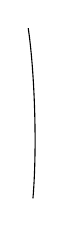
\begin{tikzpicture}[x=0.6cm,y=0.6cm]
\draw (0,0) .. controls (0.1,1.2) and (0.02,2.8) .. (-0.1,3.6);
\end{tikzpicture}}
\margin{NB. $\alpha\mapsto(\alpha'\leftrightarrow\alpha_*)$\par $\beta\mapsto(\beta'\leftrightarrow\beta_*)$}

Ceci vu, je dis que \deleted{\unsure{le}} pour $\alpha$ (ou $\alpha',\alpha_*$) donné, $\beta_*$ (ou $\beta'$) est déterminé de façon unique, par les conditions de la proposition. En effet, $\beta_*(S')$ est connu quand on connaît les $S\in\Sigma_E$ tels que $S\mid\circ\mid\beta_*(S')$, ce sont ceux pour lesquels on a $\alpha_*(S)\mid\circ\mid S'$ !

% margin note written sideways, slanted upwards to the right
\margin{\uline{\unsure{Déf}} On dit que $\alpha,\beta$ sont \inserted{\uline{pré}}transposés \unsure{l'une|l'un} de l'autre, et que $\alpha',\beta'$, ou $\alpha_*,\beta_*$ sont \uline{transposés} \unsure{l'un|l'une} de l'autre.}
% Curved separator at the lower right of the slanted margin note.
\figure{
\begin{tikzpicture}[x=0.6cm,y=0.6cm]
\draw (0,0) .. controls (-0.08,0.9) and (0.05,1.55) .. (0.55,2.05)
 -- (0.25,2.12) .. controls (0.03,2.2) and (-0.04,2.35) .. (-0.08,2.55);
\end{tikzpicture}}

Il reste à voir quelles sont les applications
\[
\alpha:E\longrightarrow\Sigma_{E'},
\]
ou ce qui revient au $=$, les applications correspondantes
\[
\alpha_*:\Sigma_E\ \unsure{\text{---}|\longrightarrow}\ \Sigma_{E'},\qquad \alpha_*(S)=\underset{x\in S}{\operatorname{Sup}_{\Sigma_{E'}}}\alpha(x)
\]
pour lesquelles il existe une $\unsure{\beta}$
\[
\beta:E'\ \unsure{\text{---}|\longrightarrow}\ \Sigma_E,
\]
\deleted{\unsure{ou ce qui revient}}\inserted{\unsure{i.e. une}}
\[
\beta_*:\Sigma_{E'}\ \unsure{\text{---}|\longrightarrow}\ \Sigma_E,\qquad \beta_*(S')=\underset{x'\in S'}{\operatorname{Sup}_{\unsure{\Sigma_E|\Sigma_{E'}}}}\beta(\unsure{x'})
\]
\unsure{transposée|transposé}.

On va quand $=$ partir de $\alpha:E\unsure{\text{---}|\longrightarrow}\unsure{\mathscr{P}|\mathcal{P}}(E')$ \unsure{ald|au lieu de} $E\unsure{\longrightarrow|\text{---}}\unsure{\Sigma|\mathscr{P}}_{E'}$.
